% ---------------------------------------------------------------------------
% Section 3 (Method) of "Procedural Reconstruction of Slender Plants from Any
% Field Modality", written to the placeholders in the 2026-10-07 draft:
%   3.1 three short paragraphs, 3.2 + Table 1, 3.3 two-three paragraphs,
%   3.4 two paragraphs, 3.5 one-two paragraphs, Fig. 1 and Fig. 2.
% % ---------------------------------------------------------------------------
% Section 3 (Method) of "Procedural Reconstruction of Slender Plants from Any
% Field Modality", written to the placeholders in the 2026-10-07 draft:
%   3.1 three short paragraphs, 3.2 + Table 1, 3.3 two-three paragraphs,
%   3.4 two paragraphs, 3.5 one-two paragraphs, Fig. 1 and Fig. 2.
% % ---------------------------------------------------------------------------
% Section 3 (Method) of "Procedural Reconstruction of Slender Plants from Any
% Field Modality", written to the placeholders in the 2026-10-07 draft:
%   3.1 three short paragraphs, 3.2 + Table 1, 3.3 two-three paragraphs,
%   3.4 two paragraphs, 3.5 one-two paragraphs, Fig. 1 and Fig. 2.
% % ---------------------------------------------------------------------------
% Section 3 (Method) of "Procedural Reconstruction of Slender Plants from Any
% Field Modality", written to the placeholders in the 2026-10-07 draft:
%   3.1 three short paragraphs, 3.2 + Table 1, 3.3 two-three paragraphs,
%   3.4 two paragraphs, 3.5 one-two paragraphs, Fig. 1 and Fig. 2.
% \input{method} where the placeholders were.  Everything stated about the
% model is what the code does (embodied_mae_4m.py, train_sorghum_4m.py,
% train_sorghum_4m_distill.py); numbers that depend on the FieldProc reruns
% are marked \todo.
%
% Macros assumed from the main file: \CropCode, \FieldProc (small caps),
% \todo (red note).  Fallbacks are provided below.
%
% Citation keys used here -> reference numbers in the draft PDF:
%   he2022mae [21]  bachmann2022multimae [3]  mizrahi2023fourm [31]
%   pang2022pointmae [33]  dong2025embodiedmae [10]  golkar2023xval [14]
%   hinton2015distill [22]  wu2021dcd [47]  song2026chamfer [42]
%   hadadi2025vlm [17]  kimara2025maizefield3d [25]  hadadi2026floraforge [20]
%   tobin2017domainrand [46]  qi2017pointnet [36]
% ---------------------------------------------------------------------------
\providecommand{\CropCode}{\textsc{CropCode}}
\providecommand{\FieldProc}{\textsc{FieldProc}}
\providecommand{\todo}[1]{\textcolor{red}{#1}}
\providecommand{\R}{\mathbb{R}}

\section{Method}
\label{sec:method}

\begin{figure*}[t]
  \centering
  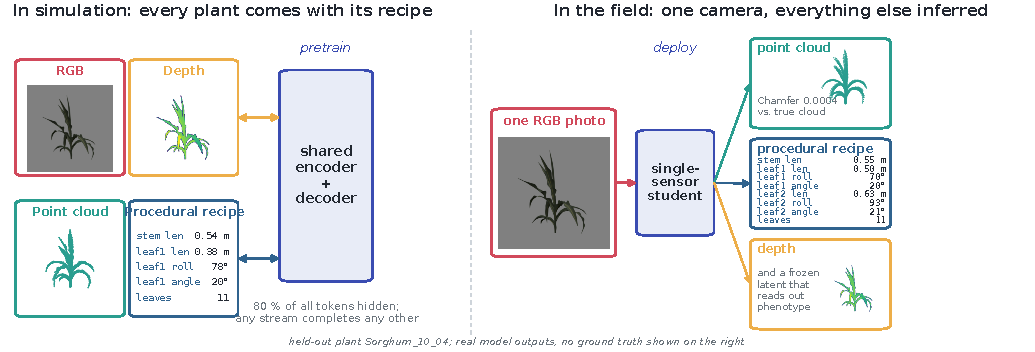
\includegraphics[width=\textwidth]{fig_teaser.pdf}
  \caption{\textbf{Any sensor in, procedural plant out.} From any subset of
  field-practical modalities (a single photograph, a depth frame, or a point
  cloud truncated by row neighbors), \CropCode{} recovers the full procedural
  representation of the plant: a kilobyte-scale, physiologically interpretable
  parameter set that re-renders to complete geometry, feeds simulation, and
  supports trait analytics at field scale. Right: real outputs of the RGB-only
  student on a held-out plant.}
  \label{fig:teaser}
\end{figure*}

\subsection{Problem formulation}
\label{sec:problem}

A procedural generator $G$ maps a parameter vector $\theta$ to a complete plant
mesh. For the crops we study $\theta$ is organ-level and interpretable: stem
length and direction, panicle geometry, and for each leaf its insertion height,
length, roll, branching angle and blade width ($d$ scalars in all;
Tab.~\ref{tab:fieldproc}). A sensor observes $G(\theta)$ only through a subset
$S\subseteq\{\mathrm{rgb},\mathrm{d},\mathrm{pc}\}$ of a photograph
$x^{\mathrm{rgb}}$, a depth frame $x^{\mathrm{d}}$, and a point cloud
$x^{\mathrm{pc}}$, from one viewpoint, with the plant's neighbors occluding part
of it. The quantities an agronomist needs---height, leaf count, blade angles,
biomass---are functions of $\theta$, not of any one observation.

The task is amortized inversion under this degradation: a single network
$f_\phi$ that, from whichever $S$ the campaign produced, returns $\hat\theta$
together with the modalities that were not observed, in one forward pass, for
thousands of plants per day. This differs from per-instance optimization
against a rich capture~\cite{hadadi2025vlm} in both its input (one fragment,
not a complete scan) and its cost (milliseconds, not minutes), and from
learned completion in its output (a program, not a point set).

Two commitments follow. First, the generator supplies both the training data
and the output representation: \CropCode{} is pretrained entirely on
$G$-rendered plants paired with their exact $\theta$, so the model's target is
the very parameterization that downstream simulation consumes. Second,
$\theta$ is available in simulation and never in the field, so at deployment
it is strictly a prediction \emph{target}; during training it may serve as
privileged information. Whether it should also enter the encoder as an input
modality during pretraining is a design question we answer empirically
(Sec.~\ref{sec:param-stream}); the formulation leaves that choice open through
a single masking ratio.

\subsection{A procedural field-data engine}
\label{sec:data}

\begin{table}[t]
  \centering\small
  \setlength{\tabcolsep}{4pt}
  \begin{tabular}{lcc}
    \toprule
     & Maize & Sorghum \\
    \midrule
    Plants & \todo{$N$} & \todo{$N$} (15{,}000 in this draft) \\
    Views / plant & 10 & 10 \\
    Parameters / plant ($d$) & $14 + 14\times28$ & $9 + 5\times24$ \\
    Leaf count range & \todo{3--22} & 4--35 \\
    Occluded-row variants & \todo{\ldots} & \todo{\ldots} \\
    Neighbor points in crop & $\sim$30\% & \todo{\ldots} \\
    Real-field eval split & \todo{MaizeField3D~\cite{kimara2025maizefield3d}} & \todo{---} \\
    \bottomrule
  \end{tabular}
  \caption{\FieldProc{} at a glance. $d$ counts the plant token plus the leaf
  tokens the model regresses. \todo{finalize $N$, diversity axes (phenotypes
  / generator configurations / growth stages) and the real-data row
  (MaizeField3D scans + pipeline GT~\cite{hadadi2025vlm,kimara2025maizefield3d}).}}
  \label{tab:fieldproc}
\end{table}

\paragraph{Generation.}
Each species has one procedural generator seeded by plant index, so a
population is one continuous distribution of morphologies with exact
parameters attached; there is no discrete genotype label, and the probes of
Sec.~\ref{sec:field} are regressions, not classifications. The sorghum
generator couples height to leaf count ($\text{stem length}=0.05\,n_{\text{leaves}}-0.001$,
$R^2{=}0.988$), which bounds what any phenotype probe on that species can
separate and is why we replicate every design finding on maize, whose four
headline traits are nearly independent (height vs.\ leaf count $r{=}0.20$).

\paragraph{Rendering and the camera rig.}
Plants are rasterized offscreen (pyrender) at $1024^2$ with a $40^\circ$
vertical field of view, a shared leaf texture, three fixed directional lights
and a uniform background that is later matted to transparency. Ten cameras per
plant sit on a Fibonacci sphere of radius 2.5\,m at elevations from
$-64^\circ$ to $+64^\circ$ with golden-angle azimuths; the rig seed is fixed,
so every plant is seen from the same ten poses. Depth is stored losslessly
(32-bit packed), and for each view the complete plant cloud is exported in that
camera's frame together with the camera pose. In the \emph{isolated} regime the
cloud is the whole plant; the \emph{row} regime (Sec.~\ref{sec:regime3}) renders
the target inside a planted row whose neighbors' leaves bend on contact, so the
cloud inside the target's crop region contains neighbor points
(Tab.~\ref{tab:fieldproc}) and the images show interleaved blades.
\todo{Row-simulation specifics (spacing, contact model, occlusion severities)
from the FieldProc generation code.}

\paragraph{Splits.}
We split by plant, 70/15/15, and enrich the held-out splits with unusual
morphologies: each plant's Mahalanobis distance from the population centroid in
standardized trait space ranks it, and val/test are drawn with probability
$\propto(\text{rank}+0.02)^2$ (median extremeness 2.03 on train vs.\ 2.76 on
val/test). Held-out $R^2$ is therefore comparable between models on a split but
not a portable absolute; we report native-unit error alongside it. Training
visits each plant once per epoch with one randomly drawn view (the same draw
for every arm of an ablation), and data-scaling arms take nested random subsets
of plants with all ten views, so a step along the data axis never changes the
view regime.

\subsection{Four-stream masked pretraining}
\label{sec:pretrain}

\begin{figure*}[t]
  \centering
  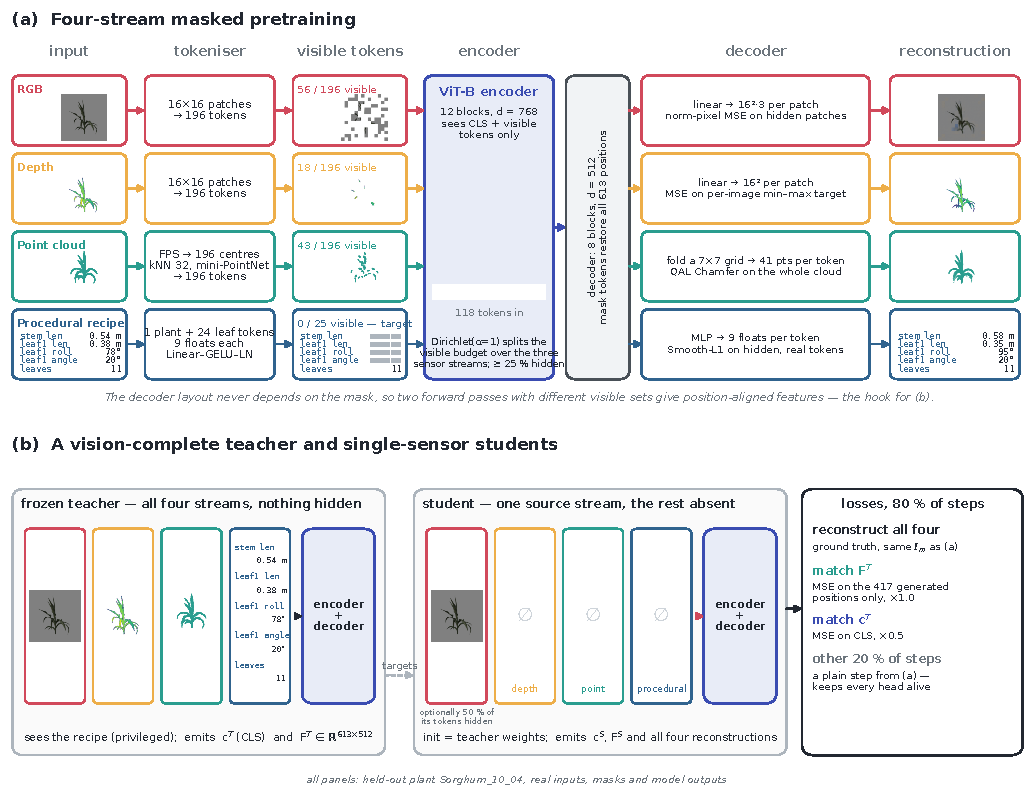
\includegraphics[width=\textwidth]{fig_architecture.pdf}
  \caption{\textbf{\CropCode{} overview.} (a)~Four token streams enter a shared
  encoder under a Dirichlet masking budget; modality-specific decoders
  reconstruct all streams. The parameter stream is decoded, never encoded
  (Sec.~\ref{sec:param-stream}). (b)~A frozen teacher shown all four streams,
  parameters included, is distilled into single-sensor students for deployment. All panels show real inputs,
  masks and model outputs for one held-out plant.}
  \label{fig:arch}
\end{figure*}

\paragraph{Tokens.}
RGB and depth are patchified into $14\times14=196$ tokens each with fixed 2-D
sine--cosine positions. The cloud is grouped Point-MAE
style~\cite{pang2022pointmae}: farthest-point sampling picks 196 centres, $k$NN
gathers 32 neighbours per centre, and a mini-PointNet~\cite{qi2017pointnet}
embeds each group relative to its centre. The parameter stream is $1+K$
\emph{number tokens}: token~0 carries the plant-level scalars and tokens
$1\ldots K$ one leaf each ($K{=}24$ sorghum, 28 maize), every field affinely
normalized to $[0,1]$ and the vector projected linearly, in the spirit of
xVal~\cite{golkar2023xval}, rather than spelled out as text; padding tokens are
flagged by a validity mask. Each token receives a learned modality embedding; a
CLS token is prepended; a 12-block ViT-B encoder ($d{=}768$) reads the visible
tokens and an 8-block decoder ($d{=}512$) restores every position of every
stream with mask tokens---$196{+}196{+}196{+}(1{+}K)$ positions in a fixed
order, independent of what was visible. Per-stream heads follow: linear
unpatchify for RGB and depth, a FoldingNet-style head that expands each PC
token into 41 points so the \emph{entire} cloud is regenerated, and an MLP that
regresses the $d$ parameters. The architecture derives from
EmbodiedMAE~\cite{dong2025embodiedmae}; the parameter stream and the masking
gate below are ours.

\paragraph{Masking.}
Let $L_m$ be the token count of modality $m$ and $\rho{=}0.80$ the total mask
ratio. Once per step we draw $\lambda\sim\mathrm{Dirichlet}(\mathbf 1)$ over
the sensor streams and allocate the visible budget
$V=\lfloor(1-\rho)\sum_m L_m\rfloor$ (117 tokens) in proportion to $\lambda$ with
exact integer counts, subject to every stream keeping at least one token and
losing at least 25\,\%; which positions are visible is drawn per sample. Counts
are shared across the batch, so no sample has an empty stream and no padding
reaches the encoder. The parameter stream is governed by a separate ratio
$\rho_\theta$: $\max(1,\lfloor(1+K)(1-\rho_\theta)\rfloor)$ of its tokens are
visible and the Dirichlet budget is allocated over the vision streams alone,
which makes the vision masks of a four-stream model bit-identical to its
three-stream sibling under the same seed. Left in the shared budget instead,
the short parameter stream is $\sim$59\,\% visible at $\rho{=}0.80$ while the
vision streams fall from 20\,\% to 18\,\%, a confound our control arms remove
(Sec.~\ref{sec:param-stream}). \CropCode{} uses $\rho_\theta{=}1$: the
parameters are reconstructed by the decoder at every step and never seen by
the encoder.

\paragraph{Objective and schedule.}
The loss sums per-stream terms over the hidden positions: per-patch-normalized
MSE for RGB~\cite{he2022mae}, MSE on a per-image min--max-normalized depth
target, Smooth-L1 (weight 5) on hidden, non-padding parameter tokens, and for
the cloud a quality-aware Chamfer on the full regenerated set,
$\ell_{\mathrm{pc}}=\frac1N\sum_i\sigma(a(d_i-\tau))\,d_i+\frac1N\sum_j\sigma(a(e_j-\tau))\,e_j$,
with $d_i,e_j$ the Euclidean nearest-neighbour distances in each direction and
a sigmoid gate ($\tau{=}0.01$, $a{=}100$) that spends gradient on residuals
above a centimetre rather than on points already on the bulk
surface~\cite{wu2021dcd,song2026chamfer}. AdamW ($\beta{=}(0.9,0.95)$, weight
decay 0.05), linear warm-up then cosine decay, gradient clipping at 1.0. The
headline model trains for 1{,}000 epochs over all views at global batch 256;
ablation arms are matched in \emph{optimizer steps} (197{,}400 at global batch
32), not epochs, because under one-view-per-plant sampling an epoch is the
plant count and equal epochs would hand a 10k-plant arm ten times the updates
of a 1k arm.

\subsection{A full-modality teacher, single-sensor students}
\label{sec:distill}

At $\rho{=}0.80$ the encoder never sees one modality standing alone with the
others entirely absent, so the pretrained model completes a single sensor only
out of distribution. We close the gap by self-distillation~\cite{hinton2015distill}
from a teacher that holds privileged information. The \emph{teacher} is the
pretrained checkpoint with the lowest validation loss, frozen, and shown
\emph{all four} streams with nothing hidden: RGB, depth, the point cloud, and
the parameter tokens themselves. Since $\theta$ is exactly what the student
must infer from a single sensor, the teacher's representation is formed with
the answer in hand, and distilling it is a learning-using-privileged-information
setting rather than plain multi-sensor to single-sensor transfer. The teacher
emits its encoder CLS latent $c^T\in\R^{768}$ and its decoder feature sequence
$F^T\in\R^{613\times512}$ after the final decoder norm; because the decoder
layout is independent of the mask, every position of $F^T$ has a student
counterpart, including the $1{+}K$ parameter positions. One caution we found
necessary: an all-visible teacher is itself out of distribution for a model
trained at $\ge$25\,\% masking per stream. On sorghum the cost is small
(full-cloud Chamfer $4.8\times10^{-4}$ all-visible vs.\ $3.5\times10^{-4}$ at
50\,\% visible per stream), but on maize the teacher's point cloud collapsed
(Chamfer $0.05$--$0.09$ vs.\ $\sim$$0.001$); there we show the teacher half of
each stream's tokens instead, and we measure a teacher's own reconstructions
before distilling from it.

The \emph{student} starts from the teacher's weights and trains for 100 epochs
(AdamW, lr $10^{-4}$, cosine, global batch 128) on two step types chosen by a
seeded coin. With probability 0.8 a \emph{single-sensor step}: one source
$s\in\{\mathrm{rgb},\mathrm{d},\mathrm{pc}\}$, cycled deterministically, is the
only stream to reach the encoder, optionally with half its own tokens hidden as
a regularizer, and the loss is
$\sum_m\ell_m+\lambda_F\,\overline{\|F^S_j-F^T_j\|^2}_{j\notin s}+\lambda_c\|c^S-c^T\|^2$
with $\lambda_F{=}1$, $\lambda_c{=}0.5$: ground-truth reconstruction of all
streams including $\theta$, plus feature matching on the positions the student
must \emph{generate}---for an RGB source, the depth, cloud and parameter
positions, where the teacher's features were computed with the parameters in
view. The student never receives parameter tokens. With probability 0.2 an ordinary masked step from
Sec.~\ref{sec:pretrain}; one such step in five is what keeps the non-target
heads alive (a depth head collapsed by $7\times$ within ten epochs without it
and recovered in one epoch with it). Specialists restrict the source list and,
optionally, the target; the generalist is one model for every $S$. Students
are scored per source with the source unmasked, against the undistilled
teacher's epoch-0 numbers measured by the same routine, since a single epoch
of distillation already captures most of the gain for some sources and
\emph{costs} ground for others.

\subsection{Crossing into the field}
\label{sec:field}

Three things separate deployment from the regime above, and the evaluation
protocol fixes each. (i)~\emph{The parameters are never observed.} Every
phenotype readout uses the frozen encoder's CLS token under
$S=\{\mathrm{rgb},\mathrm{d},\mathrm{pc}\}\cap$ (the arm's streams) with the
parameter tensor zeroed; the plant token's first field is stem length verbatim,
so any probe that exposed it would be handed the answer. The probe is ridge
regression on one deterministic view per plant, standardizer fit on train
only, scored on the extreme-enriched held-out plants with paired bootstrap
confidence intervals over plants; a modality ``wins'' only when the interval
excludes zero on val \emph{and} test. (ii)~\emph{A camera sees part of a
plant.} Training clouds are complete, so we ray-cast each view against the mesh
to mark the points a camera would actually see (one camera covers
$49\pm7\,\%$ of a sorghum plant, three cameras $78\pm4\,\%$) and score every
model under full, three-camera and one-camera clouds, both with the probe
refit per condition (information retained) and with the full-cloud probe
transferred (what a readout calibrated on complete scans does on real ones).
Reconstruction under partial input is run in the masked regime; with every
token visible the decoder is out of distribution and the cloud collapses, the
same failure that makes an unmasked teacher unsafe. (iii)~\emph{Real scans.}
We evaluate the single-sensor students on field-grown maize and sorghum whose
procedural ground truth was reconstructed independently by a staged scan
pipeline~\cite{hadadi2025vlm,kimara2025maizefield3d}, including row plots in
which neighbors occlude the target, reporting parameter error, re-rendered
geometry and the probe transfer gap of (ii) as the predicted sim-to-real
penalty. \todo{Real-split protocol: plant segmentation / matting,
camera-frame alignment of the scan, how pipeline GT handles leaves the scan
misses.}
 where the placeholders were.  Everything stated about the
% model is what the code does (embodied_mae_4m.py, train_sorghum_4m.py,
% train_sorghum_4m_distill.py); numbers that depend on the FieldProc reruns
% are marked \todo.
%
% Macros assumed from the main file: \CropCode, \FieldProc (small caps),
% \todo (red note).  Fallbacks are provided below.
%
% Citation keys used here -> reference numbers in the draft PDF:
%   he2022mae [21]  bachmann2022multimae [3]  mizrahi2023fourm [31]
%   pang2022pointmae [33]  dong2025embodiedmae [10]  golkar2023xval [14]
%   hinton2015distill [22]  wu2021dcd [47]  song2026chamfer [42]
%   hadadi2025vlm [17]  kimara2025maizefield3d [25]  hadadi2026floraforge [20]
%   tobin2017domainrand [46]  qi2017pointnet [36]
% ---------------------------------------------------------------------------
\providecommand{\CropCode}{\textsc{CropCode}}
\providecommand{\FieldProc}{\textsc{FieldProc}}
\providecommand{\todo}[1]{\textcolor{red}{#1}}
\providecommand{\R}{\mathbb{R}}

\section{Method}
\label{sec:method}

\begin{figure*}[t]
  \centering
  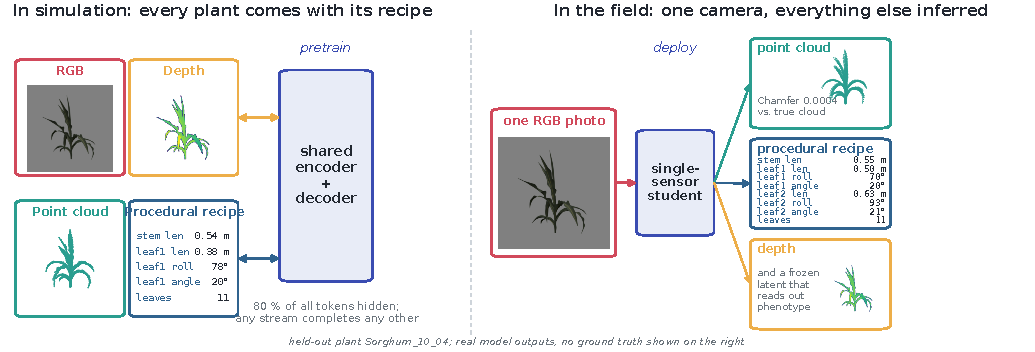
\includegraphics[width=\textwidth]{fig_teaser.pdf}
  \caption{\textbf{Any sensor in, procedural plant out.} From any subset of
  field-practical modalities (a single photograph, a depth frame, or a point
  cloud truncated by row neighbors), \CropCode{} recovers the full procedural
  representation of the plant: a kilobyte-scale, physiologically interpretable
  parameter set that re-renders to complete geometry, feeds simulation, and
  supports trait analytics at field scale. Right: real outputs of the RGB-only
  student on a held-out plant.}
  \label{fig:teaser}
\end{figure*}

\subsection{Problem formulation}
\label{sec:problem}

A procedural generator $G$ maps a parameter vector $\theta$ to a complete plant
mesh. For the crops we study $\theta$ is organ-level and interpretable: stem
length and direction, panicle geometry, and for each leaf its insertion height,
length, roll, branching angle and blade width ($d$ scalars in all;
Tab.~\ref{tab:fieldproc}). A sensor observes $G(\theta)$ only through a subset
$S\subseteq\{\mathrm{rgb},\mathrm{d},\mathrm{pc}\}$ of a photograph
$x^{\mathrm{rgb}}$, a depth frame $x^{\mathrm{d}}$, and a point cloud
$x^{\mathrm{pc}}$, from one viewpoint, with the plant's neighbors occluding part
of it. The quantities an agronomist needs---height, leaf count, blade angles,
biomass---are functions of $\theta$, not of any one observation.

The task is amortized inversion under this degradation: a single network
$f_\phi$ that, from whichever $S$ the campaign produced, returns $\hat\theta$
together with the modalities that were not observed, in one forward pass, for
thousands of plants per day. This differs from per-instance optimization
against a rich capture~\cite{hadadi2025vlm} in both its input (one fragment,
not a complete scan) and its cost (milliseconds, not minutes), and from
learned completion in its output (a program, not a point set).

Two commitments follow. First, the generator supplies both the training data
and the output representation: \CropCode{} is pretrained entirely on
$G$-rendered plants paired with their exact $\theta$, so the model's target is
the very parameterization that downstream simulation consumes. Second,
$\theta$ is available in simulation and never in the field, so at deployment
it is strictly a prediction \emph{target}; during training it may serve as
privileged information. Whether it should also enter the encoder as an input
modality during pretraining is a design question we answer empirically
(Sec.~\ref{sec:param-stream}); the formulation leaves that choice open through
a single masking ratio.

\subsection{A procedural field-data engine}
\label{sec:data}

\begin{table}[t]
  \centering\small
  \setlength{\tabcolsep}{4pt}
  \begin{tabular}{lcc}
    \toprule
     & Maize & Sorghum \\
    \midrule
    Plants & \todo{$N$} & \todo{$N$} (15{,}000 in this draft) \\
    Views / plant & 10 & 10 \\
    Parameters / plant ($d$) & $14 + 14\times28$ & $9 + 5\times24$ \\
    Leaf count range & \todo{3--22} & 4--35 \\
    Occluded-row variants & \todo{\ldots} & \todo{\ldots} \\
    Neighbor points in crop & $\sim$30\% & \todo{\ldots} \\
    Real-field eval split & \todo{MaizeField3D~\cite{kimara2025maizefield3d}} & \todo{---} \\
    \bottomrule
  \end{tabular}
  \caption{\FieldProc{} at a glance. $d$ counts the plant token plus the leaf
  tokens the model regresses. \todo{finalize $N$, diversity axes (phenotypes
  / generator configurations / growth stages) and the real-data row
  (MaizeField3D scans + pipeline GT~\cite{hadadi2025vlm,kimara2025maizefield3d}).}}
  \label{tab:fieldproc}
\end{table}

\paragraph{Generation.}
Each species has one procedural generator seeded by plant index, so a
population is one continuous distribution of morphologies with exact
parameters attached; there is no discrete genotype label, and the probes of
Sec.~\ref{sec:field} are regressions, not classifications. The sorghum
generator couples height to leaf count ($\text{stem length}=0.05\,n_{\text{leaves}}-0.001$,
$R^2{=}0.988$), which bounds what any phenotype probe on that species can
separate and is why we replicate every design finding on maize, whose four
headline traits are nearly independent (height vs.\ leaf count $r{=}0.20$).

\paragraph{Rendering and the camera rig.}
Plants are rasterized offscreen (pyrender) at $1024^2$ with a $40^\circ$
vertical field of view, a shared leaf texture, three fixed directional lights
and a uniform background that is later matted to transparency. Ten cameras per
plant sit on a Fibonacci sphere of radius 2.5\,m at elevations from
$-64^\circ$ to $+64^\circ$ with golden-angle azimuths; the rig seed is fixed,
so every plant is seen from the same ten poses. Depth is stored losslessly
(32-bit packed), and for each view the complete plant cloud is exported in that
camera's frame together with the camera pose. In the \emph{isolated} regime the
cloud is the whole plant; the \emph{row} regime (Sec.~\ref{sec:regime3}) renders
the target inside a planted row whose neighbors' leaves bend on contact, so the
cloud inside the target's crop region contains neighbor points
(Tab.~\ref{tab:fieldproc}) and the images show interleaved blades.
\todo{Row-simulation specifics (spacing, contact model, occlusion severities)
from the FieldProc generation code.}

\paragraph{Splits.}
We split by plant, 70/15/15, and enrich the held-out splits with unusual
morphologies: each plant's Mahalanobis distance from the population centroid in
standardized trait space ranks it, and val/test are drawn with probability
$\propto(\text{rank}+0.02)^2$ (median extremeness 2.03 on train vs.\ 2.76 on
val/test). Held-out $R^2$ is therefore comparable between models on a split but
not a portable absolute; we report native-unit error alongside it. Training
visits each plant once per epoch with one randomly drawn view (the same draw
for every arm of an ablation), and data-scaling arms take nested random subsets
of plants with all ten views, so a step along the data axis never changes the
view regime.

\subsection{Four-stream masked pretraining}
\label{sec:pretrain}

\begin{figure*}[t]
  \centering
  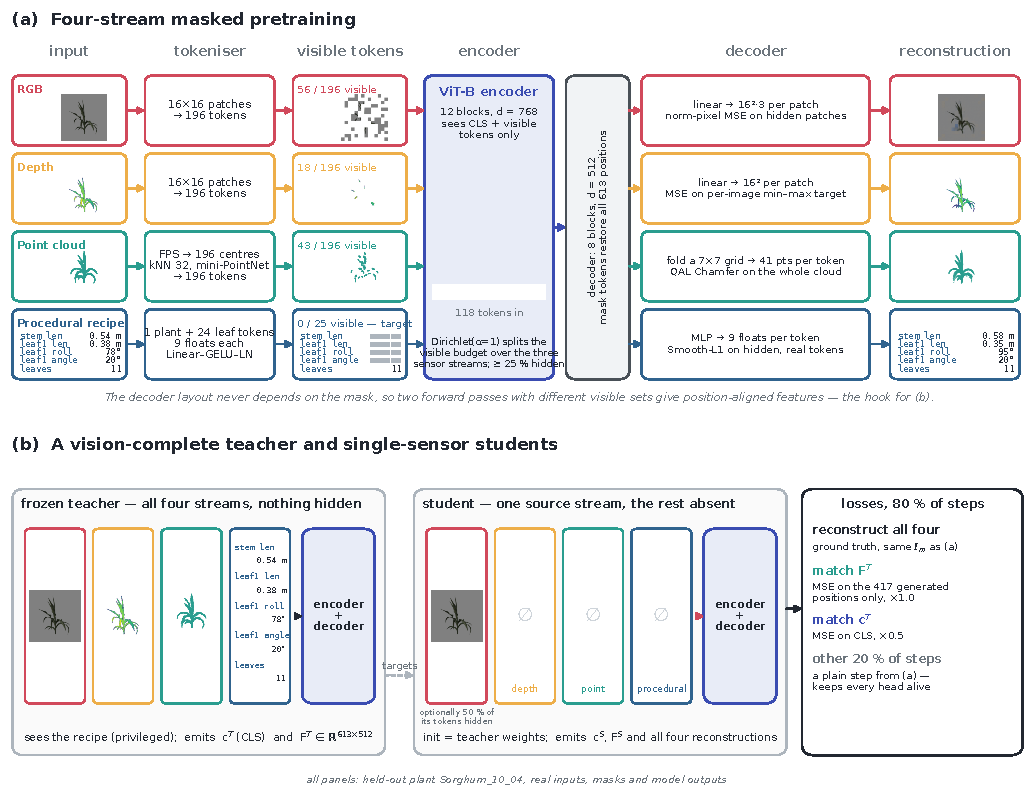
\includegraphics[width=\textwidth]{fig_architecture.pdf}
  \caption{\textbf{\CropCode{} overview.} (a)~Four token streams enter a shared
  encoder under a Dirichlet masking budget; modality-specific decoders
  reconstruct all streams. The parameter stream is decoded, never encoded
  (Sec.~\ref{sec:param-stream}). (b)~A frozen teacher shown all four streams,
  parameters included, is distilled into single-sensor students for deployment. All panels show real inputs,
  masks and model outputs for one held-out plant.}
  \label{fig:arch}
\end{figure*}

\paragraph{Tokens.}
RGB and depth are patchified into $14\times14=196$ tokens each with fixed 2-D
sine--cosine positions. The cloud is grouped Point-MAE
style~\cite{pang2022pointmae}: farthest-point sampling picks 196 centres, $k$NN
gathers 32 neighbours per centre, and a mini-PointNet~\cite{qi2017pointnet}
embeds each group relative to its centre. The parameter stream is $1+K$
\emph{number tokens}: token~0 carries the plant-level scalars and tokens
$1\ldots K$ one leaf each ($K{=}24$ sorghum, 28 maize), every field affinely
normalized to $[0,1]$ and the vector projected linearly, in the spirit of
xVal~\cite{golkar2023xval}, rather than spelled out as text; padding tokens are
flagged by a validity mask. Each token receives a learned modality embedding; a
CLS token is prepended; a 12-block ViT-B encoder ($d{=}768$) reads the visible
tokens and an 8-block decoder ($d{=}512$) restores every position of every
stream with mask tokens---$196{+}196{+}196{+}(1{+}K)$ positions in a fixed
order, independent of what was visible. Per-stream heads follow: linear
unpatchify for RGB and depth, a FoldingNet-style head that expands each PC
token into 41 points so the \emph{entire} cloud is regenerated, and an MLP that
regresses the $d$ parameters. The architecture derives from
EmbodiedMAE~\cite{dong2025embodiedmae}; the parameter stream and the masking
gate below are ours.

\paragraph{Masking.}
Let $L_m$ be the token count of modality $m$ and $\rho{=}0.80$ the total mask
ratio. Once per step we draw $\lambda\sim\mathrm{Dirichlet}(\mathbf 1)$ over
the sensor streams and allocate the visible budget
$V=\lfloor(1-\rho)\sum_m L_m\rfloor$ (117 tokens) in proportion to $\lambda$ with
exact integer counts, subject to every stream keeping at least one token and
losing at least 25\,\%; which positions are visible is drawn per sample. Counts
are shared across the batch, so no sample has an empty stream and no padding
reaches the encoder. The parameter stream is governed by a separate ratio
$\rho_\theta$: $\max(1,\lfloor(1+K)(1-\rho_\theta)\rfloor)$ of its tokens are
visible and the Dirichlet budget is allocated over the vision streams alone,
which makes the vision masks of a four-stream model bit-identical to its
three-stream sibling under the same seed. Left in the shared budget instead,
the short parameter stream is $\sim$59\,\% visible at $\rho{=}0.80$ while the
vision streams fall from 20\,\% to 18\,\%, a confound our control arms remove
(Sec.~\ref{sec:param-stream}). \CropCode{} uses $\rho_\theta{=}1$: the
parameters are reconstructed by the decoder at every step and never seen by
the encoder.

\paragraph{Objective and schedule.}
The loss sums per-stream terms over the hidden positions: per-patch-normalized
MSE for RGB~\cite{he2022mae}, MSE on a per-image min--max-normalized depth
target, Smooth-L1 (weight 5) on hidden, non-padding parameter tokens, and for
the cloud a quality-aware Chamfer on the full regenerated set,
$\ell_{\mathrm{pc}}=\frac1N\sum_i\sigma(a(d_i-\tau))\,d_i+\frac1N\sum_j\sigma(a(e_j-\tau))\,e_j$,
with $d_i,e_j$ the Euclidean nearest-neighbour distances in each direction and
a sigmoid gate ($\tau{=}0.01$, $a{=}100$) that spends gradient on residuals
above a centimetre rather than on points already on the bulk
surface~\cite{wu2021dcd,song2026chamfer}. AdamW ($\beta{=}(0.9,0.95)$, weight
decay 0.05), linear warm-up then cosine decay, gradient clipping at 1.0. The
headline model trains for 1{,}000 epochs over all views at global batch 256;
ablation arms are matched in \emph{optimizer steps} (197{,}400 at global batch
32), not epochs, because under one-view-per-plant sampling an epoch is the
plant count and equal epochs would hand a 10k-plant arm ten times the updates
of a 1k arm.

\subsection{A full-modality teacher, single-sensor students}
\label{sec:distill}

At $\rho{=}0.80$ the encoder never sees one modality standing alone with the
others entirely absent, so the pretrained model completes a single sensor only
out of distribution. We close the gap by self-distillation~\cite{hinton2015distill}
from a teacher that holds privileged information. The \emph{teacher} is the
pretrained checkpoint with the lowest validation loss, frozen, and shown
\emph{all four} streams with nothing hidden: RGB, depth, the point cloud, and
the parameter tokens themselves. Since $\theta$ is exactly what the student
must infer from a single sensor, the teacher's representation is formed with
the answer in hand, and distilling it is a learning-using-privileged-information
setting rather than plain multi-sensor to single-sensor transfer. The teacher
emits its encoder CLS latent $c^T\in\R^{768}$ and its decoder feature sequence
$F^T\in\R^{613\times512}$ after the final decoder norm; because the decoder
layout is independent of the mask, every position of $F^T$ has a student
counterpart, including the $1{+}K$ parameter positions. One caution we found
necessary: an all-visible teacher is itself out of distribution for a model
trained at $\ge$25\,\% masking per stream. On sorghum the cost is small
(full-cloud Chamfer $4.8\times10^{-4}$ all-visible vs.\ $3.5\times10^{-4}$ at
50\,\% visible per stream), but on maize the teacher's point cloud collapsed
(Chamfer $0.05$--$0.09$ vs.\ $\sim$$0.001$); there we show the teacher half of
each stream's tokens instead, and we measure a teacher's own reconstructions
before distilling from it.

The \emph{student} starts from the teacher's weights and trains for 100 epochs
(AdamW, lr $10^{-4}$, cosine, global batch 128) on two step types chosen by a
seeded coin. With probability 0.8 a \emph{single-sensor step}: one source
$s\in\{\mathrm{rgb},\mathrm{d},\mathrm{pc}\}$, cycled deterministically, is the
only stream to reach the encoder, optionally with half its own tokens hidden as
a regularizer, and the loss is
$\sum_m\ell_m+\lambda_F\,\overline{\|F^S_j-F^T_j\|^2}_{j\notin s}+\lambda_c\|c^S-c^T\|^2$
with $\lambda_F{=}1$, $\lambda_c{=}0.5$: ground-truth reconstruction of all
streams including $\theta$, plus feature matching on the positions the student
must \emph{generate}---for an RGB source, the depth, cloud and parameter
positions, where the teacher's features were computed with the parameters in
view. The student never receives parameter tokens. With probability 0.2 an ordinary masked step from
Sec.~\ref{sec:pretrain}; one such step in five is what keeps the non-target
heads alive (a depth head collapsed by $7\times$ within ten epochs without it
and recovered in one epoch with it). Specialists restrict the source list and,
optionally, the target; the generalist is one model for every $S$. Students
are scored per source with the source unmasked, against the undistilled
teacher's epoch-0 numbers measured by the same routine, since a single epoch
of distillation already captures most of the gain for some sources and
\emph{costs} ground for others.

\subsection{Crossing into the field}
\label{sec:field}

Three things separate deployment from the regime above, and the evaluation
protocol fixes each. (i)~\emph{The parameters are never observed.} Every
phenotype readout uses the frozen encoder's CLS token under
$S=\{\mathrm{rgb},\mathrm{d},\mathrm{pc}\}\cap$ (the arm's streams) with the
parameter tensor zeroed; the plant token's first field is stem length verbatim,
so any probe that exposed it would be handed the answer. The probe is ridge
regression on one deterministic view per plant, standardizer fit on train
only, scored on the extreme-enriched held-out plants with paired bootstrap
confidence intervals over plants; a modality ``wins'' only when the interval
excludes zero on val \emph{and} test. (ii)~\emph{A camera sees part of a
plant.} Training clouds are complete, so we ray-cast each view against the mesh
to mark the points a camera would actually see (one camera covers
$49\pm7\,\%$ of a sorghum plant, three cameras $78\pm4\,\%$) and score every
model under full, three-camera and one-camera clouds, both with the probe
refit per condition (information retained) and with the full-cloud probe
transferred (what a readout calibrated on complete scans does on real ones).
Reconstruction under partial input is run in the masked regime; with every
token visible the decoder is out of distribution and the cloud collapses, the
same failure that makes an unmasked teacher unsafe. (iii)~\emph{Real scans.}
We evaluate the single-sensor students on field-grown maize and sorghum whose
procedural ground truth was reconstructed independently by a staged scan
pipeline~\cite{hadadi2025vlm,kimara2025maizefield3d}, including row plots in
which neighbors occlude the target, reporting parameter error, re-rendered
geometry and the probe transfer gap of (ii) as the predicted sim-to-real
penalty. \todo{Real-split protocol: plant segmentation / matting,
camera-frame alignment of the scan, how pipeline GT handles leaves the scan
misses.}
 where the placeholders were.  Everything stated about the
% model is what the code does (embodied_mae_4m.py, train_sorghum_4m.py,
% train_sorghum_4m_distill.py); numbers that depend on the FieldProc reruns
% are marked \todo.
%
% Macros assumed from the main file: \CropCode, \FieldProc (small caps),
% \todo (red note).  Fallbacks are provided below.
%
% Citation keys used here -> reference numbers in the draft PDF:
%   he2022mae [21]  bachmann2022multimae [3]  mizrahi2023fourm [31]
%   pang2022pointmae [33]  dong2025embodiedmae [10]  golkar2023xval [14]
%   hinton2015distill [22]  wu2021dcd [47]  song2026chamfer [42]
%   hadadi2025vlm [17]  kimara2025maizefield3d [25]  hadadi2026floraforge [20]
%   tobin2017domainrand [46]  qi2017pointnet [36]
% ---------------------------------------------------------------------------
\providecommand{\CropCode}{\textsc{CropCode}}
\providecommand{\FieldProc}{\textsc{FieldProc}}
\providecommand{\todo}[1]{\textcolor{red}{#1}}
\providecommand{\R}{\mathbb{R}}

\section{Method}
\label{sec:method}

\begin{figure*}[t]
  \centering
  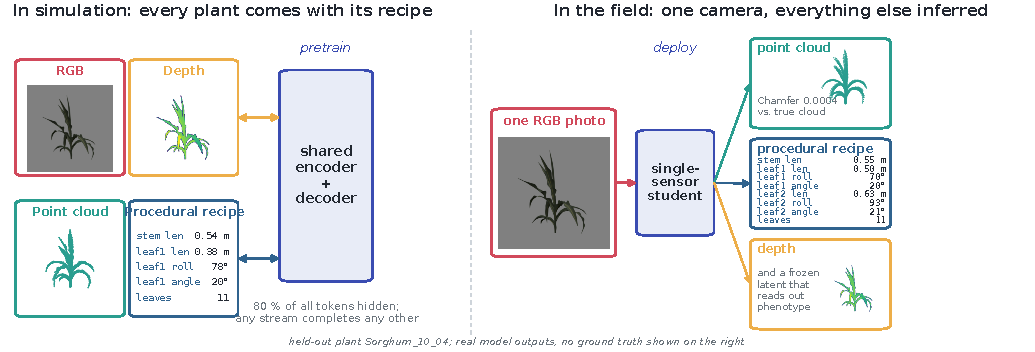
\includegraphics[width=\textwidth]{fig_teaser.pdf}
  \caption{\textbf{Any sensor in, procedural plant out.} From any subset of
  field-practical modalities (a single photograph, a depth frame, or a point
  cloud truncated by row neighbors), \CropCode{} recovers the full procedural
  representation of the plant: a kilobyte-scale, physiologically interpretable
  parameter set that re-renders to complete geometry, feeds simulation, and
  supports trait analytics at field scale. Right: real outputs of the RGB-only
  student on a held-out plant.}
  \label{fig:teaser}
\end{figure*}

\subsection{Problem formulation}
\label{sec:problem}

A procedural generator $G$ maps a parameter vector $\theta$ to a complete plant
mesh. For the crops we study $\theta$ is organ-level and interpretable: stem
length and direction, panicle geometry, and for each leaf its insertion height,
length, roll, branching angle and blade width ($d$ scalars in all;
Tab.~\ref{tab:fieldproc}). A sensor observes $G(\theta)$ only through a subset
$S\subseteq\{\mathrm{rgb},\mathrm{d},\mathrm{pc}\}$ of a photograph
$x^{\mathrm{rgb}}$, a depth frame $x^{\mathrm{d}}$, and a point cloud
$x^{\mathrm{pc}}$, from one viewpoint, with the plant's neighbors occluding part
of it. The quantities an agronomist needs---height, leaf count, blade angles,
biomass---are functions of $\theta$, not of any one observation.

The task is amortized inversion under this degradation: a single network
$f_\phi$ that, from whichever $S$ the campaign produced, returns $\hat\theta$
together with the modalities that were not observed, in one forward pass, for
thousands of plants per day. This differs from per-instance optimization
against a rich capture~\cite{hadadi2025vlm} in both its input (one fragment,
not a complete scan) and its cost (milliseconds, not minutes), and from
learned completion in its output (a program, not a point set).

Two commitments follow. First, the generator supplies both the training data
and the output representation: \CropCode{} is pretrained entirely on
$G$-rendered plants paired with their exact $\theta$, so the model's target is
the very parameterization that downstream simulation consumes. Second,
$\theta$ is available in simulation and never in the field, so at deployment
it is strictly a prediction \emph{target}; during training it may serve as
privileged information. Whether it should also enter the encoder as an input
modality during pretraining is a design question we answer empirically
(Sec.~\ref{sec:param-stream}); the formulation leaves that choice open through
a single masking ratio.

\subsection{A procedural field-data engine}
\label{sec:data}

\begin{table}[t]
  \centering\small
  \setlength{\tabcolsep}{4pt}
  \begin{tabular}{lcc}
    \toprule
     & Maize & Sorghum \\
    \midrule
    Plants & \todo{$N$} & \todo{$N$} (15{,}000 in this draft) \\
    Views / plant & 10 & 10 \\
    Parameters / plant ($d$) & $14 + 14\times28$ & $9 + 5\times24$ \\
    Leaf count range & \todo{3--22} & 4--35 \\
    Occluded-row variants & \todo{\ldots} & \todo{\ldots} \\
    Neighbor points in crop & $\sim$30\% & \todo{\ldots} \\
    Real-field eval split & \todo{MaizeField3D~\cite{kimara2025maizefield3d}} & \todo{---} \\
    \bottomrule
  \end{tabular}
  \caption{\FieldProc{} at a glance. $d$ counts the plant token plus the leaf
  tokens the model regresses. \todo{finalize $N$, diversity axes (phenotypes
  / generator configurations / growth stages) and the real-data row
  (MaizeField3D scans + pipeline GT~\cite{hadadi2025vlm,kimara2025maizefield3d}).}}
  \label{tab:fieldproc}
\end{table}

\paragraph{Generation.}
Each species has one procedural generator seeded by plant index, so a
population is one continuous distribution of morphologies with exact
parameters attached; there is no discrete genotype label, and the probes of
Sec.~\ref{sec:field} are regressions, not classifications. The sorghum
generator couples height to leaf count ($\text{stem length}=0.05\,n_{\text{leaves}}-0.001$,
$R^2{=}0.988$), which bounds what any phenotype probe on that species can
separate and is why we replicate every design finding on maize, whose four
headline traits are nearly independent (height vs.\ leaf count $r{=}0.20$).

\paragraph{Rendering and the camera rig.}
Plants are rasterized offscreen (pyrender) at $1024^2$ with a $40^\circ$
vertical field of view, a shared leaf texture, three fixed directional lights
and a uniform background that is later matted to transparency. Ten cameras per
plant sit on a Fibonacci sphere of radius 2.5\,m at elevations from
$-64^\circ$ to $+64^\circ$ with golden-angle azimuths; the rig seed is fixed,
so every plant is seen from the same ten poses. Depth is stored losslessly
(32-bit packed), and for each view the complete plant cloud is exported in that
camera's frame together with the camera pose. In the \emph{isolated} regime the
cloud is the whole plant; the \emph{row} regime (Sec.~\ref{sec:regime3}) renders
the target inside a planted row whose neighbors' leaves bend on contact, so the
cloud inside the target's crop region contains neighbor points
(Tab.~\ref{tab:fieldproc}) and the images show interleaved blades.
\todo{Row-simulation specifics (spacing, contact model, occlusion severities)
from the FieldProc generation code.}

\paragraph{Splits.}
We split by plant, 70/15/15, and enrich the held-out splits with unusual
morphologies: each plant's Mahalanobis distance from the population centroid in
standardized trait space ranks it, and val/test are drawn with probability
$\propto(\text{rank}+0.02)^2$ (median extremeness 2.03 on train vs.\ 2.76 on
val/test). Held-out $R^2$ is therefore comparable between models on a split but
not a portable absolute; we report native-unit error alongside it. Training
visits each plant once per epoch with one randomly drawn view (the same draw
for every arm of an ablation), and data-scaling arms take nested random subsets
of plants with all ten views, so a step along the data axis never changes the
view regime.

\subsection{Four-stream masked pretraining}
\label{sec:pretrain}

\begin{figure*}[t]
  \centering
  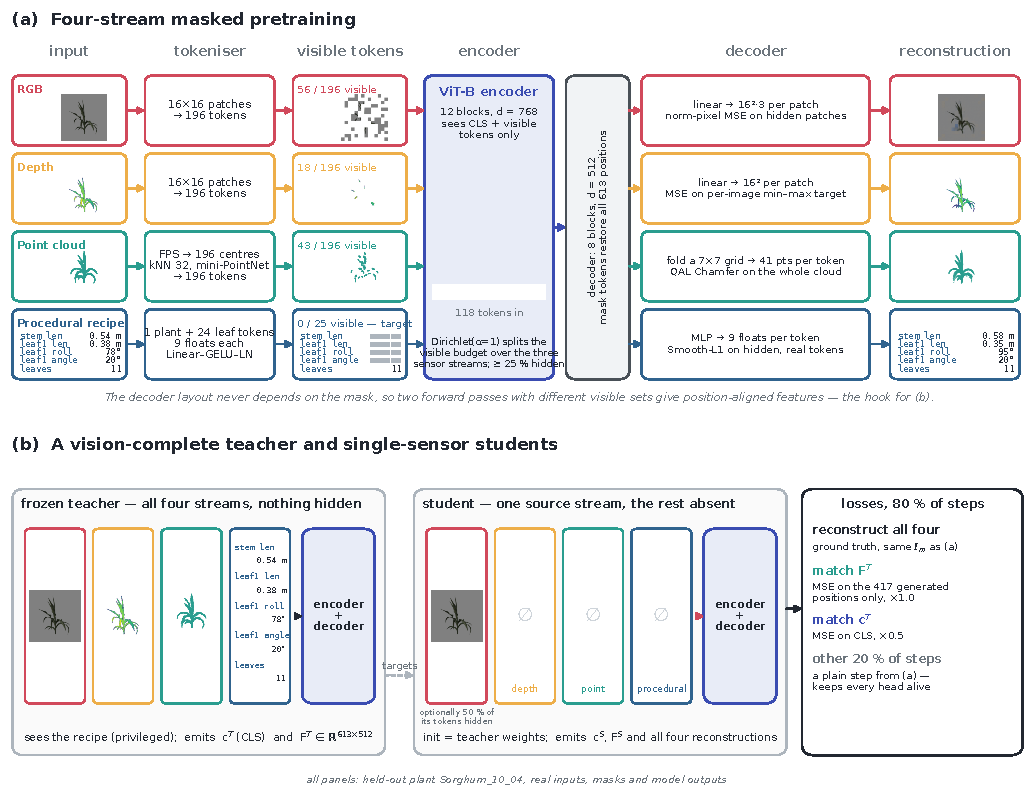
\includegraphics[width=\textwidth]{fig_architecture.pdf}
  \caption{\textbf{\CropCode{} overview.} (a)~Four token streams enter a shared
  encoder under a Dirichlet masking budget; modality-specific decoders
  reconstruct all streams. The parameter stream is decoded, never encoded
  (Sec.~\ref{sec:param-stream}). (b)~A frozen teacher shown all four streams,
  parameters included, is distilled into single-sensor students for deployment. All panels show real inputs,
  masks and model outputs for one held-out plant.}
  \label{fig:arch}
\end{figure*}

\paragraph{Tokens.}
RGB and depth are patchified into $14\times14=196$ tokens each with fixed 2-D
sine--cosine positions. The cloud is grouped Point-MAE
style~\cite{pang2022pointmae}: farthest-point sampling picks 196 centres, $k$NN
gathers 32 neighbours per centre, and a mini-PointNet~\cite{qi2017pointnet}
embeds each group relative to its centre. The parameter stream is $1+K$
\emph{number tokens}: token~0 carries the plant-level scalars and tokens
$1\ldots K$ one leaf each ($K{=}24$ sorghum, 28 maize), every field affinely
normalized to $[0,1]$ and the vector projected linearly, in the spirit of
xVal~\cite{golkar2023xval}, rather than spelled out as text; padding tokens are
flagged by a validity mask. Each token receives a learned modality embedding; a
CLS token is prepended; a 12-block ViT-B encoder ($d{=}768$) reads the visible
tokens and an 8-block decoder ($d{=}512$) restores every position of every
stream with mask tokens---$196{+}196{+}196{+}(1{+}K)$ positions in a fixed
order, independent of what was visible. Per-stream heads follow: linear
unpatchify for RGB and depth, a FoldingNet-style head that expands each PC
token into 41 points so the \emph{entire} cloud is regenerated, and an MLP that
regresses the $d$ parameters. The architecture derives from
EmbodiedMAE~\cite{dong2025embodiedmae}; the parameter stream and the masking
gate below are ours.

\paragraph{Masking.}
Let $L_m$ be the token count of modality $m$ and $\rho{=}0.80$ the total mask
ratio. Once per step we draw $\lambda\sim\mathrm{Dirichlet}(\mathbf 1)$ over
the sensor streams and allocate the visible budget
$V=\lfloor(1-\rho)\sum_m L_m\rfloor$ (117 tokens) in proportion to $\lambda$ with
exact integer counts, subject to every stream keeping at least one token and
losing at least 25\,\%; which positions are visible is drawn per sample. Counts
are shared across the batch, so no sample has an empty stream and no padding
reaches the encoder. The parameter stream is governed by a separate ratio
$\rho_\theta$: $\max(1,\lfloor(1+K)(1-\rho_\theta)\rfloor)$ of its tokens are
visible and the Dirichlet budget is allocated over the vision streams alone,
which makes the vision masks of a four-stream model bit-identical to its
three-stream sibling under the same seed. Left in the shared budget instead,
the short parameter stream is $\sim$59\,\% visible at $\rho{=}0.80$ while the
vision streams fall from 20\,\% to 18\,\%, a confound our control arms remove
(Sec.~\ref{sec:param-stream}). \CropCode{} uses $\rho_\theta{=}1$: the
parameters are reconstructed by the decoder at every step and never seen by
the encoder.

\paragraph{Objective and schedule.}
The loss sums per-stream terms over the hidden positions: per-patch-normalized
MSE for RGB~\cite{he2022mae}, MSE on a per-image min--max-normalized depth
target, Smooth-L1 (weight 5) on hidden, non-padding parameter tokens, and for
the cloud a quality-aware Chamfer on the full regenerated set,
$\ell_{\mathrm{pc}}=\frac1N\sum_i\sigma(a(d_i-\tau))\,d_i+\frac1N\sum_j\sigma(a(e_j-\tau))\,e_j$,
with $d_i,e_j$ the Euclidean nearest-neighbour distances in each direction and
a sigmoid gate ($\tau{=}0.01$, $a{=}100$) that spends gradient on residuals
above a centimetre rather than on points already on the bulk
surface~\cite{wu2021dcd,song2026chamfer}. AdamW ($\beta{=}(0.9,0.95)$, weight
decay 0.05), linear warm-up then cosine decay, gradient clipping at 1.0. The
headline model trains for 1{,}000 epochs over all views at global batch 256;
ablation arms are matched in \emph{optimizer steps} (197{,}400 at global batch
32), not epochs, because under one-view-per-plant sampling an epoch is the
plant count and equal epochs would hand a 10k-plant arm ten times the updates
of a 1k arm.

\subsection{A full-modality teacher, single-sensor students}
\label{sec:distill}

At $\rho{=}0.80$ the encoder never sees one modality standing alone with the
others entirely absent, so the pretrained model completes a single sensor only
out of distribution. We close the gap by self-distillation~\cite{hinton2015distill}
from a teacher that holds privileged information. The \emph{teacher} is the
pretrained checkpoint with the lowest validation loss, frozen, and shown
\emph{all four} streams with nothing hidden: RGB, depth, the point cloud, and
the parameter tokens themselves. Since $\theta$ is exactly what the student
must infer from a single sensor, the teacher's representation is formed with
the answer in hand, and distilling it is a learning-using-privileged-information
setting rather than plain multi-sensor to single-sensor transfer. The teacher
emits its encoder CLS latent $c^T\in\R^{768}$ and its decoder feature sequence
$F^T\in\R^{613\times512}$ after the final decoder norm; because the decoder
layout is independent of the mask, every position of $F^T$ has a student
counterpart, including the $1{+}K$ parameter positions. One caution we found
necessary: an all-visible teacher is itself out of distribution for a model
trained at $\ge$25\,\% masking per stream. On sorghum the cost is small
(full-cloud Chamfer $4.8\times10^{-4}$ all-visible vs.\ $3.5\times10^{-4}$ at
50\,\% visible per stream), but on maize the teacher's point cloud collapsed
(Chamfer $0.05$--$0.09$ vs.\ $\sim$$0.001$); there we show the teacher half of
each stream's tokens instead, and we measure a teacher's own reconstructions
before distilling from it.

The \emph{student} starts from the teacher's weights and trains for 100 epochs
(AdamW, lr $10^{-4}$, cosine, global batch 128) on two step types chosen by a
seeded coin. With probability 0.8 a \emph{single-sensor step}: one source
$s\in\{\mathrm{rgb},\mathrm{d},\mathrm{pc}\}$, cycled deterministically, is the
only stream to reach the encoder, optionally with half its own tokens hidden as
a regularizer, and the loss is
$\sum_m\ell_m+\lambda_F\,\overline{\|F^S_j-F^T_j\|^2}_{j\notin s}+\lambda_c\|c^S-c^T\|^2$
with $\lambda_F{=}1$, $\lambda_c{=}0.5$: ground-truth reconstruction of all
streams including $\theta$, plus feature matching on the positions the student
must \emph{generate}---for an RGB source, the depth, cloud and parameter
positions, where the teacher's features were computed with the parameters in
view. The student never receives parameter tokens. With probability 0.2 an ordinary masked step from
Sec.~\ref{sec:pretrain}; one such step in five is what keeps the non-target
heads alive (a depth head collapsed by $7\times$ within ten epochs without it
and recovered in one epoch with it). Specialists restrict the source list and,
optionally, the target; the generalist is one model for every $S$. Students
are scored per source with the source unmasked, against the undistilled
teacher's epoch-0 numbers measured by the same routine, since a single epoch
of distillation already captures most of the gain for some sources and
\emph{costs} ground for others.

\subsection{Crossing into the field}
\label{sec:field}

Three things separate deployment from the regime above, and the evaluation
protocol fixes each. (i)~\emph{The parameters are never observed.} Every
phenotype readout uses the frozen encoder's CLS token under
$S=\{\mathrm{rgb},\mathrm{d},\mathrm{pc}\}\cap$ (the arm's streams) with the
parameter tensor zeroed; the plant token's first field is stem length verbatim,
so any probe that exposed it would be handed the answer. The probe is ridge
regression on one deterministic view per plant, standardizer fit on train
only, scored on the extreme-enriched held-out plants with paired bootstrap
confidence intervals over plants; a modality ``wins'' only when the interval
excludes zero on val \emph{and} test. (ii)~\emph{A camera sees part of a
plant.} Training clouds are complete, so we ray-cast each view against the mesh
to mark the points a camera would actually see (one camera covers
$49\pm7\,\%$ of a sorghum plant, three cameras $78\pm4\,\%$) and score every
model under full, three-camera and one-camera clouds, both with the probe
refit per condition (information retained) and with the full-cloud probe
transferred (what a readout calibrated on complete scans does on real ones).
Reconstruction under partial input is run in the masked regime; with every
token visible the decoder is out of distribution and the cloud collapses, the
same failure that makes an unmasked teacher unsafe. (iii)~\emph{Real scans.}
We evaluate the single-sensor students on field-grown maize and sorghum whose
procedural ground truth was reconstructed independently by a staged scan
pipeline~\cite{hadadi2025vlm,kimara2025maizefield3d}, including row plots in
which neighbors occlude the target, reporting parameter error, re-rendered
geometry and the probe transfer gap of (ii) as the predicted sim-to-real
penalty. \todo{Real-split protocol: plant segmentation / matting,
camera-frame alignment of the scan, how pipeline GT handles leaves the scan
misses.}
 where the placeholders were.  Everything stated about the
% model is what the code does (embodied_mae_4m.py, train_sorghum_4m.py,
% train_sorghum_4m_distill.py); numbers that depend on the FieldProc reruns
% are marked \todo.
%
% Macros assumed from the main file: \CropCode, \FieldProc (small caps),
% \todo (red note).  Fallbacks are provided below.
%
% Citation keys used here -> reference numbers in the draft PDF:
%   he2022mae [21]  bachmann2022multimae [3]  mizrahi2023fourm [31]
%   pang2022pointmae [33]  dong2025embodiedmae [10]  golkar2023xval [14]
%   hinton2015distill [22]  wu2021dcd [47]  song2026chamfer [42]
%   hadadi2025vlm [17]  kimara2025maizefield3d [25]  hadadi2026floraforge [20]
%   tobin2017domainrand [46]  qi2017pointnet [36]
% ---------------------------------------------------------------------------
\providecommand{\CropCode}{\textsc{CropCode}}
\providecommand{\FieldProc}{\textsc{FieldProc}}
\providecommand{\todo}[1]{\textcolor{red}{#1}}
\providecommand{\R}{\mathbb{R}}

\section{Method}
\label{sec:method}

\begin{figure*}[t]
  \centering
  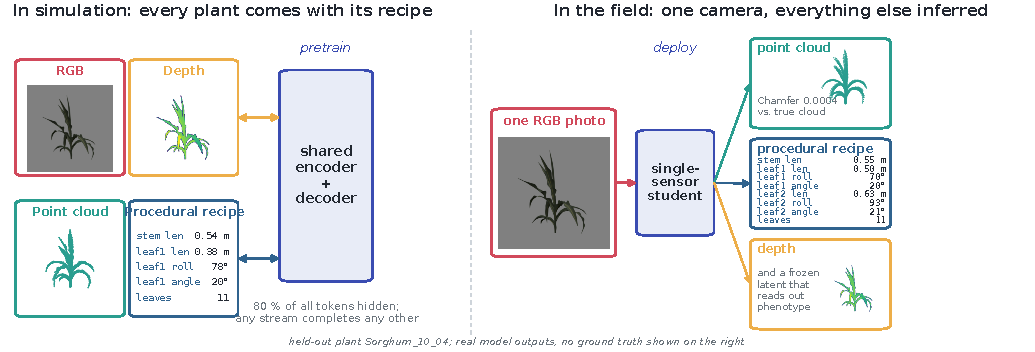
\includegraphics[width=\textwidth]{fig_teaser.pdf}
  \caption{\textbf{Any sensor in, procedural plant out.} From any subset of
  field-practical modalities (a single photograph, a depth frame, or a point
  cloud truncated by row neighbors), \CropCode{} recovers the full procedural
  representation of the plant: a kilobyte-scale, physiologically interpretable
  parameter set that re-renders to complete geometry, feeds simulation, and
  supports trait analytics at field scale. Right: real outputs of the RGB-only
  student on a held-out plant.}
  \label{fig:teaser}
\end{figure*}

\subsection{Problem formulation}
\label{sec:problem}

A procedural generator $G$ maps a parameter vector $\theta$ to a complete plant
mesh. For the crops we study $\theta$ is organ-level and interpretable: stem
length and direction, panicle geometry, and for each leaf its insertion height,
length, roll, branching angle and blade width ($d$ scalars in all;
Tab.~\ref{tab:fieldproc}). A sensor observes $G(\theta)$ only through a subset
$S\subseteq\{\mathrm{rgb},\mathrm{d},\mathrm{pc}\}$ of a photograph
$x^{\mathrm{rgb}}$, a depth frame $x^{\mathrm{d}}$, and a point cloud
$x^{\mathrm{pc}}$, from one viewpoint, with the plant's neighbors occluding part
of it. The quantities an agronomist needs---height, leaf count, blade angles,
biomass---are functions of $\theta$, not of any one observation.

The task is amortized inversion under this degradation: a single network
$f_\phi$ that, from whichever $S$ the campaign produced, returns $\hat\theta$
together with the modalities that were not observed, in one forward pass, for
thousands of plants per day. This differs from per-instance optimization
against a rich capture~\cite{hadadi2025vlm} in both its input (one fragment,
not a complete scan) and its cost (milliseconds, not minutes), and from
learned completion in its output (a program, not a point set).

Two commitments follow. First, the generator supplies both the training data
and the output representation: \CropCode{} is pretrained entirely on
$G$-rendered plants paired with their exact $\theta$, so the model's target is
the very parameterization that downstream simulation consumes. Second,
$\theta$ is available in simulation and never in the field, so at deployment
it is strictly a prediction \emph{target}; during training it may serve as
privileged information. Whether it should also enter the encoder as an input
modality during pretraining is a design question we answer empirically
(Sec.~\ref{sec:param-stream}); the formulation leaves that choice open through
a single masking ratio.

\subsection{A procedural field-data engine}
\label{sec:data}

\begin{table}[t]
  \centering\small
  \setlength{\tabcolsep}{4pt}
  \begin{tabular}{lcc}
    \toprule
     & Maize & Sorghum \\
    \midrule
    Plants & \todo{$N$} & \todo{$N$} (15{,}000 in this draft) \\
    Views / plant & 10 & 10 \\
    Parameters / plant ($d$) & $14 + 14\times28$ & $9 + 5\times24$ \\
    Leaf count range & \todo{3--22} & 4--35 \\
    Occluded-row variants & \todo{\ldots} & \todo{\ldots} \\
    Neighbor points in crop & $\sim$30\% & \todo{\ldots} \\
    Real-field eval split & \todo{MaizeField3D~\cite{kimara2025maizefield3d}} & \todo{---} \\
    \bottomrule
  \end{tabular}
  \caption{\FieldProc{} at a glance. $d$ counts the plant token plus the leaf
  tokens the model regresses. \todo{finalize $N$, diversity axes (phenotypes
  / generator configurations / growth stages) and the real-data row
  (MaizeField3D scans + pipeline GT~\cite{hadadi2025vlm,kimara2025maizefield3d}).}}
  \label{tab:fieldproc}
\end{table}

\paragraph{Generation.}
Each species has one procedural generator seeded by plant index, so a
population is one continuous distribution of morphologies with exact
parameters attached; there is no discrete genotype label, and the probes of
Sec.~\ref{sec:field} are regressions, not classifications. The sorghum
generator couples height to leaf count ($\text{stem length}=0.05\,n_{\text{leaves}}-0.001$,
$R^2{=}0.988$), which bounds what any phenotype probe on that species can
separate and is why we replicate every design finding on maize, whose four
headline traits are nearly independent (height vs.\ leaf count $r{=}0.20$).

\paragraph{Rendering and the camera rig.}
Plants are rasterized offscreen (pyrender) at $1024^2$ with a $40^\circ$
vertical field of view, a shared leaf texture, three fixed directional lights
and a uniform background that is later matted to transparency. Ten cameras per
plant sit on a Fibonacci sphere of radius 2.5\,m at elevations from
$-64^\circ$ to $+64^\circ$ with golden-angle azimuths; the rig seed is fixed,
so every plant is seen from the same ten poses. Depth is stored losslessly
(32-bit packed), and for each view the complete plant cloud is exported in that
camera's frame together with the camera pose. In the \emph{isolated} regime the
cloud is the whole plant; the \emph{row} regime (Sec.~\ref{sec:regime3}) renders
the target inside a planted row whose neighbors' leaves bend on contact, so the
cloud inside the target's crop region contains neighbor points
(Tab.~\ref{tab:fieldproc}) and the images show interleaved blades.
\todo{Row-simulation specifics (spacing, contact model, occlusion severities)
from the FieldProc generation code.}

\paragraph{Splits.}
We split by plant, 70/15/15, and enrich the held-out splits with unusual
morphologies: each plant's Mahalanobis distance from the population centroid in
standardized trait space ranks it, and val/test are drawn with probability
$\propto(\text{rank}+0.02)^2$ (median extremeness 2.03 on train vs.\ 2.76 on
val/test). Held-out $R^2$ is therefore comparable between models on a split but
not a portable absolute; we report native-unit error alongside it. Training
visits each plant once per epoch with one randomly drawn view (the same draw
for every arm of an ablation), and data-scaling arms take nested random subsets
of plants with all ten views, so a step along the data axis never changes the
view regime.

\subsection{Four-stream masked pretraining}
\label{sec:pretrain}

\begin{figure*}[t]
  \centering
  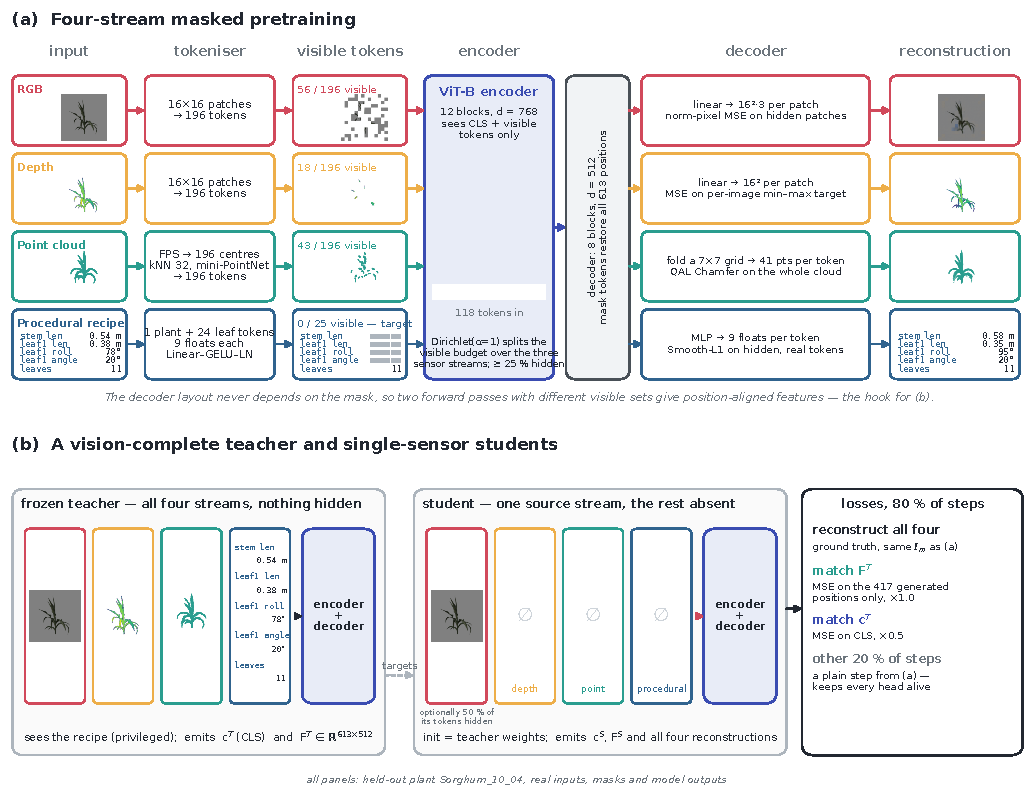
\includegraphics[width=\textwidth]{fig_architecture.pdf}
  \caption{\textbf{\CropCode{} overview.} (a)~Four token streams enter a shared
  encoder under a Dirichlet masking budget; modality-specific decoders
  reconstruct all streams. The parameter stream is decoded, never encoded
  (Sec.~\ref{sec:param-stream}). (b)~A frozen teacher shown all four streams,
  parameters included, is distilled into single-sensor students for deployment. All panels show real inputs,
  masks and model outputs for one held-out plant.}
  \label{fig:arch}
\end{figure*}

\paragraph{Tokens.}
RGB and depth are patchified into $14\times14=196$ tokens each with fixed 2-D
sine--cosine positions. The cloud is grouped Point-MAE
style~\cite{pang2022pointmae}: farthest-point sampling picks 196 centres, $k$NN
gathers 32 neighbours per centre, and a mini-PointNet~\cite{qi2017pointnet}
embeds each group relative to its centre. The parameter stream is $1+K$
\emph{number tokens}: token~0 carries the plant-level scalars and tokens
$1\ldots K$ one leaf each ($K{=}24$ sorghum, 28 maize), every field affinely
normalized to $[0,1]$ and the vector projected linearly, in the spirit of
xVal~\cite{golkar2023xval}, rather than spelled out as text; padding tokens are
flagged by a validity mask. Each token receives a learned modality embedding; a
CLS token is prepended; a 12-block ViT-B encoder ($d{=}768$) reads the visible
tokens and an 8-block decoder ($d{=}512$) restores every position of every
stream with mask tokens---$196{+}196{+}196{+}(1{+}K)$ positions in a fixed
order, independent of what was visible. Per-stream heads follow: linear
unpatchify for RGB and depth, a FoldingNet-style head that expands each PC
token into 41 points so the \emph{entire} cloud is regenerated, and an MLP that
regresses the $d$ parameters. The architecture derives from
EmbodiedMAE~\cite{dong2025embodiedmae}; the parameter stream and the masking
gate below are ours.

\paragraph{Masking.}
Let $L_m$ be the token count of modality $m$ and $\rho{=}0.80$ the total mask
ratio. Once per step we draw $\lambda\sim\mathrm{Dirichlet}(\mathbf 1)$ over
the sensor streams and allocate the visible budget
$V=\lfloor(1-\rho)\sum_m L_m\rfloor$ (117 tokens) in proportion to $\lambda$ with
exact integer counts, subject to every stream keeping at least one token and
losing at least 25\,\%; which positions are visible is drawn per sample. Counts
are shared across the batch, so no sample has an empty stream and no padding
reaches the encoder. The parameter stream is governed by a separate ratio
$\rho_\theta$: $\max(1,\lfloor(1+K)(1-\rho_\theta)\rfloor)$ of its tokens are
visible and the Dirichlet budget is allocated over the vision streams alone,
which makes the vision masks of a four-stream model bit-identical to its
three-stream sibling under the same seed. Left in the shared budget instead,
the short parameter stream is $\sim$59\,\% visible at $\rho{=}0.80$ while the
vision streams fall from 20\,\% to 18\,\%, a confound our control arms remove
(Sec.~\ref{sec:param-stream}). \CropCode{} uses $\rho_\theta{=}1$: the
parameters are reconstructed by the decoder at every step and never seen by
the encoder.

\paragraph{Objective and schedule.}
The loss sums per-stream terms over the hidden positions: per-patch-normalized
MSE for RGB~\cite{he2022mae}, MSE on a per-image min--max-normalized depth
target, Smooth-L1 (weight 5) on hidden, non-padding parameter tokens, and for
the cloud a quality-aware Chamfer on the full regenerated set,
$\ell_{\mathrm{pc}}=\frac1N\sum_i\sigma(a(d_i-\tau))\,d_i+\frac1N\sum_j\sigma(a(e_j-\tau))\,e_j$,
with $d_i,e_j$ the Euclidean nearest-neighbour distances in each direction and
a sigmoid gate ($\tau{=}0.01$, $a{=}100$) that spends gradient on residuals
above a centimetre rather than on points already on the bulk
surface~\cite{wu2021dcd,song2026chamfer}. AdamW ($\beta{=}(0.9,0.95)$, weight
decay 0.05), linear warm-up then cosine decay, gradient clipping at 1.0. The
headline model trains for 1{,}000 epochs over all views at global batch 256;
ablation arms are matched in \emph{optimizer steps} (197{,}400 at global batch
32), not epochs, because under one-view-per-plant sampling an epoch is the
plant count and equal epochs would hand a 10k-plant arm ten times the updates
of a 1k arm.

\subsection{A full-modality teacher, single-sensor students}
\label{sec:distill}

At $\rho{=}0.80$ the encoder never sees one modality standing alone with the
others entirely absent, so the pretrained model completes a single sensor only
out of distribution. We close the gap by self-distillation~\cite{hinton2015distill}
from a teacher that holds privileged information. The \emph{teacher} is the
pretrained checkpoint with the lowest validation loss, frozen, and shown
\emph{all four} streams with nothing hidden: RGB, depth, the point cloud, and
the parameter tokens themselves. Since $\theta$ is exactly what the student
must infer from a single sensor, the teacher's representation is formed with
the answer in hand, and distilling it is a learning-using-privileged-information
setting rather than plain multi-sensor to single-sensor transfer. The teacher
emits its encoder CLS latent $c^T\in\R^{768}$ and its decoder feature sequence
$F^T\in\R^{613\times512}$ after the final decoder norm; because the decoder
layout is independent of the mask, every position of $F^T$ has a student
counterpart, including the $1{+}K$ parameter positions. One caution we found
necessary: an all-visible teacher is itself out of distribution for a model
trained at $\ge$25\,\% masking per stream. On sorghum the cost is small
(full-cloud Chamfer $4.8\times10^{-4}$ all-visible vs.\ $3.5\times10^{-4}$ at
50\,\% visible per stream), but on maize the teacher's point cloud collapsed
(Chamfer $0.05$--$0.09$ vs.\ $\sim$$0.001$); there we show the teacher half of
each stream's tokens instead, and we measure a teacher's own reconstructions
before distilling from it.

The \emph{student} starts from the teacher's weights and trains for 100 epochs
(AdamW, lr $10^{-4}$, cosine, global batch 128) on two step types chosen by a
seeded coin. With probability 0.8 a \emph{single-sensor step}: one source
$s\in\{\mathrm{rgb},\mathrm{d},\mathrm{pc}\}$, cycled deterministically, is the
only stream to reach the encoder, optionally with half its own tokens hidden as
a regularizer, and the loss is
$\sum_m\ell_m+\lambda_F\,\overline{\|F^S_j-F^T_j\|^2}_{j\notin s}+\lambda_c\|c^S-c^T\|^2$
with $\lambda_F{=}1$, $\lambda_c{=}0.5$: ground-truth reconstruction of all
streams including $\theta$, plus feature matching on the positions the student
must \emph{generate}---for an RGB source, the depth, cloud and parameter
positions, where the teacher's features were computed with the parameters in
view. The student never receives parameter tokens. With probability 0.2 an ordinary masked step from
Sec.~\ref{sec:pretrain}; one such step in five is what keeps the non-target
heads alive (a depth head collapsed by $7\times$ within ten epochs without it
and recovered in one epoch with it). Specialists restrict the source list and,
optionally, the target; the generalist is one model for every $S$. Students
are scored per source with the source unmasked, against the undistilled
teacher's epoch-0 numbers measured by the same routine, since a single epoch
of distillation already captures most of the gain for some sources and
\emph{costs} ground for others.

\subsection{Crossing into the field}
\label{sec:field}

Three things separate deployment from the regime above, and the evaluation
protocol fixes each. (i)~\emph{The parameters are never observed.} Every
phenotype readout uses the frozen encoder's CLS token under
$S=\{\mathrm{rgb},\mathrm{d},\mathrm{pc}\}\cap$ (the arm's streams) with the
parameter tensor zeroed; the plant token's first field is stem length verbatim,
so any probe that exposed it would be handed the answer. The probe is ridge
regression on one deterministic view per plant, standardizer fit on train
only, scored on the extreme-enriched held-out plants with paired bootstrap
confidence intervals over plants; a modality ``wins'' only when the interval
excludes zero on val \emph{and} test. (ii)~\emph{A camera sees part of a
plant.} Training clouds are complete, so we ray-cast each view against the mesh
to mark the points a camera would actually see (one camera covers
$49\pm7\,\%$ of a sorghum plant, three cameras $78\pm4\,\%$) and score every
model under full, three-camera and one-camera clouds, both with the probe
refit per condition (information retained) and with the full-cloud probe
transferred (what a readout calibrated on complete scans does on real ones).
Reconstruction under partial input is run in the masked regime; with every
token visible the decoder is out of distribution and the cloud collapses, the
same failure that makes an unmasked teacher unsafe. (iii)~\emph{Real scans.}
We evaluate the single-sensor students on field-grown maize and sorghum whose
procedural ground truth was reconstructed independently by a staged scan
pipeline~\cite{hadadi2025vlm,kimara2025maizefield3d}, including row plots in
which neighbors occlude the target, reporting parameter error, re-rendered
geometry and the probe transfer gap of (ii) as the predicted sim-to-real
penalty. \todo{Real-split protocol: plant segmentation / matting,
camera-frame alignment of the scan, how pipeline GT handles leaves the scan
misses.}
